% !TEX root=../meca1321-synthesis.tex

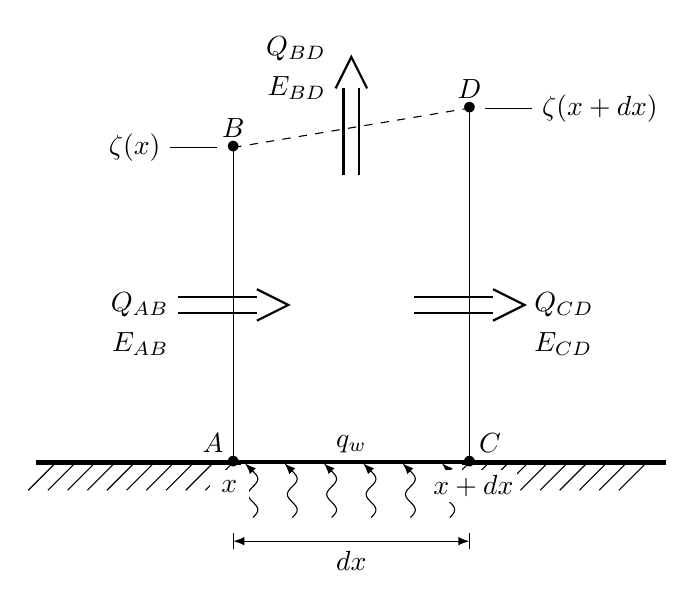
\begin{tikzpicture}
  % Tracé des parois
  \draw [ultra thick] (-4,-1) -- (4,-1);
  \foreach \i in {0,..., 9,10,21,22,...,30}
  {
    \pgfmathsetmacro{\x}{(- 4 + \i/4)};
    \draw (\x+1/4,-1) -- ++(-135:0.5);
  }
  \draw (-1.5, -1) node {$\bullet$};
  \draw ( 1.5, -1) node {$\bullet$};
  \fill (-1.4, -1.025) [white] rectangle (1.4, -1.8);
  %Repères et autres flèches
  \foreach \i in {0,...,5}
  {
    \pgfmathsetmacro{\y}{(-1.25 + \i/2)};
    \draw [domain=0:3*pi] plot ({sin(deg(\x))/16 + \y}, {\x/16-1.7}) [>=latex, ->] -- ++(-0.1,0.1);
  }
  \draw (0, -1) node [above] {$q_w$};
  \fill (-1.8, -1.1) [white] rectangle (-1.3, -1.5);
  \draw (-1.55, -1.3) node {$x$};
  \fill (1 , -1.1) [white] rectangle (2.1, -1.5);
  \draw (1.55,-1.3) node {$x+dx$};

  \draw (-1.5, -1) node [above left] {$A$} -- (-1.5, 3) node {$\bullet$} node [above] {$B$};
  \draw (-1.5, 3) [dashed] -- (1.5, 3.5) node {$\bullet$} node [above] {$D$};
  \draw (1.5, 3.5) -- (1.5, -1) node [above right] {$C$};

  \draw (0.8, 0.9) [thick] -- (1.8, 0.9);
  \draw (0.8, 1.1) [thick] -- (1.8, 1.1);
  \draw (1.8, 0.8) [thick]-- (2.2, 1) -- (1.8, 1.2);

  \draw (-2.2, 0.9) [thick] -- (-1.2, 0.9);
  \draw (-2.2, 1.1) [thick] -- (-1.2, 1.1);
  \draw (-1.2, 0.8) [thick] -- (-0.8, 1) -- (-1.2, 1.2);

  \draw (-0.1, 2.65) [thick] -- (-0.1, 3.75);
  \draw (0.1, 2.65) [thick] -- (0.1, 3.75);
  \draw (-0.2, 3.75) [thick] -- (0, 4.15) -- (0.2, 3.75);

  \draw (-2.2, 1) node [left] {$Q_{AB}$};
  \draw (-2.2, 0.5) node [left] {$E_{AB}$};

  \draw (2.2, 1) node [right] {$Q_{CD}$};
  \draw (2.2, 0.5) node [right] {$E_{CD}$};

  \draw (-0.2, 3.75) node [left] {$E_{BD}$};
  \draw (-0.2, 4.25) node [left] {$Q_{BD}$};

  \draw (-1.7, 3) -- (-2.3, 3) node [left] {$\zeta(x)$};
  \draw (1.7, 3.5) -- (2.3, 3.5) node [right] {$\zeta(x + dx)$};

  \draw (-1.5, -2) [>=latex,<->]-- (1.5, -2);
  \draw (-1.5, -2.1) -- (-1.5, -1.9);
  \draw (1.5, -2.1) -- (1.5, -1.9);
  \draw (0, -2) node [below] {$dx$};

\end{tikzpicture}
